\documentclass[a4paper,9pt,oneside,openany,article,twocolumn]{memoir}
\usepackage{amsfonts}
\usepackage{amsmath}
\usepackage[dutch]{babel}
\usepackage[pdfborder={0 0 0}]{hyperref}
\usepackage{minted}
\usepackage[wordspacing=normal,tracking=normal,charwidths=normal,leading=normal]{savetrees}

% fonts
\usepackage[T1]{fontenc}
\usepackage[charter]{mathdesign}
\usepackage[scaled]{beramono,berasans}
\usepackage{microtype}

% colors
\definecolor{uablue}{RGB}{0,61,100}
\definecolor{uared}{RGB}{126,0,47}
\definecolor{vividbrown}{RGB}{215,154,70}
\definecolor{uagreen}{RGB}{0,126,17}

\newcommand\fnurl[2]{%
  \href{#2}{#1}\footnote{\url{#2}}%
}

\author{Pieter Belmans}
\title{Een \LaTeX-vademecum}

\chapterstyle{article}
\counterwithout{section}{chapter}

\begin{document}
\maketitle

\section{Basisdocument}
Je begint altijd van volgend basisdocument:
\begin{minted}[frame=lines]{tex}
\documentclass[a4paper]{article}
\usepackage[dutch]{babel}
\usepackage{hyperref}

\author{Naam}
\title{Titel}

\begin{document}
\maketitle

\end{document}
\end{minted}
Alle commando's tussen \mint{tex}|\documentclass[a4paper]{article}| en \mint{tex}|\begin{document}| vormen de \emph{preamble}, terwijl alles tussen \mint{tex}|\begin{document}| en \mint{tex}|\end{document}| het eigenlijke document is. In de preamble komen de packages en de configuratie van je bestand, in het document je tekst.


\section{Witruimte}
\begin{enumerate}
  \item \'e\'en spatie is hetzelfde als meerdere spaties;
  \item spaties, tabs en enters zijn (bijna) hetzelfde;
  \item spaties aan het begin van een regel worden volledig genegeerd;
  \item twee regeleindes, dus \'e\'en witregel is een nieuwe alinea.
\end{enumerate}


\section{Speciale karakters}
Sommige karakters in \LaTeX\ zijn niet zomaar te produceren, je moet ze \emph{escapen}.

\begin{center}
  \begin{tabular}{cccccccc}
    \mint{tex}|\$| & \$ & 
    \mint{tex}|\&| & \& &
    \mint{tex}|\%| & \% &
    \mint{tex}|\#| & \# \\
    \mint{tex}|\_| & \_ &
    \mint{tex}|\{| & \{ &
    \mint{tex}|\}| & \}
  \end{tabular}
\end{center}

Ook voor aanhalingstekens is het opletten geblazen: gebruik \verb|``tekst''| in plaats van \verb|"tekst"|. Dit geldt ook voor \verb|`enkele'|. Daarnaast zijn er vier liggende streepjes:
\begin{center}
  \begin{tabular}[]{cccc}
  	naam & input & output & doel \\\midrule
    hyphen & \mint{tex}|-| & - & splitsen in lettergrepen \\
  	en dash & \mint{tex}|--| & -- & reeksen jaartallen, pagina's, \ldots \\
  	em dash & \mint{tex}|---| & --- & gedachtestreepje \\
  	minteken & \mint{tex}|$-$| & $-$ & in wiskundige uitdrukking
  \end{tabular}
\end{center}


\section{Structuur}
Je maakt een nieuwe alinea door een witregel open te laten, \emph{niet} door creatief gebruik van \mint{tex}|\\|. Om hoofdstukken en varianten aan te duiden gebruiken we
\begin{center}
  \begin{tabular}{lcl}
    commando & niveau & opmerking \\\midrule
    \mint{tex}|\part{}| & -1 & niet in~\texttt{letter} \\
    \mint{tex}|\chapter{}| & 0 & niet in~\texttt{letter} en~\texttt{article} \\
    \mint{tex}|\section{}| & 1 & niet in~\texttt{letter} \\
    \mint{tex}|\subsection{}| & 2 & niet in~\texttt{letter} \\
    \mint{tex}|\subsubsection{}| & 3 & niet in~\texttt{letter} \\
    \mint{tex}|\paragraph{}| & 4 & niet in~\texttt{letter} \\
    \mint{tex}|\subparagraph{}| & 5 & niet in~\texttt{letter} \\
  \end{tabular}
\end{center}

En gebruik \mint{tex}|\tableofcontents| om een inhoudstafel te produceren. Als je niet wil dat een bepaald hoofdstuk hier in komt: \mint{tex}|\section*{}|, de zogeheten \emph{starred variant}. Om te verwijzen:
\begin{minted}[frame=lines]{tex}
\section{Een interessante titel}
\label{interessant}

...

In Hoofdstuk~\ref{interessant} zagen we dat...
Op pagina~\pageref{interessant} zagen we dat...
\end{minted}

Voetnoten doen we via \mint{tex}|\footnote{}|,

\section{Stijlen}
\begin{center}
  \begin{tabular}{ll}
    commando & resultaat \\\midrule
    \mint{tex}|\emph{}| & \emph{benadrukte tekst} \\[3pt]
    \mint{tex}|\textsl{}| & \textsl{slanted tekst} \\
    \mint{tex}|\textit{}| & \textit{italic tekst} \\
    \mint{tex}|\textbf{}| & \textbf{vette tekst} \\
    \mint{tex}|\textsf{}| & \textsf{sans-serif tekst} \\
    \mint{tex}|\texttt{}| & \texttt{typewriter tekst} \\
    \mint{tex}!\verb||! & \verb|verbatim !\%|
  \end{tabular}
\end{center}


\section{Lettergroottes}
We passen het \emph{globaal} aan als optie voor de \verb|documentclass|, dus~\mint{tex}|\documentclass[11pt]{article}|. Om \emph{lokaal} te wijzigen:
\begin{center}
  \begin{tabular}{llll}
    grootte & 10pt (default) & 11pt optie & 12pt optie \\\midrule
    \mint{tex}|\tiny|         &	6.80565  &	7.33325  & 7.33325  \\
    \mint{tex}|\scriptsize|   & 7.97224  &	8.50012  & 8.50012  \\
    \mint{tex}|\footnotesize| & 8.50012  &	9.24994  & 10.00002 \\
    \mint{tex}|\small|        & 9.24994  &	10.00002 & 10.95003 \\
    \mint{tex}|\normalsize|   & 10.00002 &	10.95003 & 11.74988 \\
    \mint{tex}|\large|        & 11.74988 &	11.74988 & 14.09984 \\
    \mint{tex}|\Large|        & 14.09984 &	14.09984 & 15.84985 \\
    \mint{tex}|\LARGE|        & 15.84985 &	15.84985 & 19.02350 \\
    \mint{tex}|\huge|         & 19.02350 &	19.02350 & 22.82086 \\
    \mint{tex}|\Huge|         & 22.82086 &	22.82086 & 22.82086 \\
  \end{tabular}
\end{center}
Om dit te gebruiken plaatsen we accolades \emph{rond} de tekst die we willen wijzigen, met het commando \emph{tussen} de haakjes. Een voorbeeldje
\begin{minted}[frame=lines]{tex}
Dit is {\small kleine} tekst.
Dit is {\LARGE al behoorlijk groot}.  
\end{minted}


\section{Lettertypes}
Enkel globaal wijzigen! Lokaal \emph{kan}, maar is moeilijker en af te raden. Voor een overzicht, zie \fnurl{de \TeX\ User Group catalogus}{http://www.tug.dk/FontCatalogue}. Een paar voorbeeldjes:
\begin{minted}[frame=lines]{tex}
\usepackage[T1]{fontenc}
\usepackage[charter]{mathdesign}
\usepackage[scaled]{beramono,berasans}

\usepackage[T1]{fontenc}
\usepackage{tgpagella}
\usepackage{mathpazo}
\end{minted}
En \mint{tex}|\usepackage{microtype}| is altijd een goed idee.


\section{Opsommingen}
\begin{minted}[frame=lines]{tex}
\begin{enumerate}
  \item tekst
  \item meer tekst
\end{enumerate}
\end{minted}

\begin{minted}[frame=lines]{tex}
\begin{itemize}
  \item tekst
  \item meer tekst
\end{itemize}
\end{minted}

\begin{minted}[frame=lines]{tex}
\begin{description}
  \item[label] definitie
  \item[label] definitie
\end{description}
\end{minted}


\section{Bibliografie}
In een \verb|document.bib| bestand voeg je de bibliografie-informatie toe:
\begin{minted}[frame=lines]{text}
@book{formalized-music,
  author = {Iannis Xenakis},
  title = {Formalized Music}
  publisher = {Pendragon Press},
  year = {2001},
  edition = {2},
  isbn = {978-1576470794},
}
\end{minted}
Voor een overzicht van alle velden etc.\ gebruik ik altijd \fnurl{Wikibooks}{http://en.wikibooks.org/wiki/LaTeX/Bibliography_Management}.

In je eigenlijke document (dat in dezelfde map staat) doe je vervolgens:
\begin{minted}[frame=lines]{tex}
\cite{formalized-music}

\bibliographystyle{plain}
\bibliography{document}
\end{minted}
Er zijn de standaardstijlen \verb|plain|, \verb|abbrv| en \verb|alpha|. Zie bijvoorbeeld \fnurl{\textsf{natbib}}{http://ctan.org/pkg/natbib} voor meer mogelijkheden.


\section{Tabellen en figuren}
Altijd \mint{tex}|\usepackage{graphicx}| toevoegen voor afbeeldingen te kunnen gebruiken. Enkele voorbeelden van afbeeldingen en tabellen:
\begin{minted}[frame=lines]{tex}
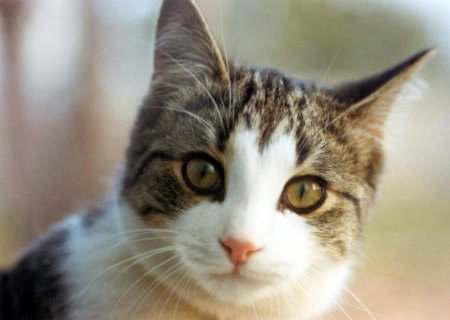
\includegraphics[width=5cm]{cat.jpg}
\begin{tabular}{l|cr}
  links & gecentreerd & rechts \\ \hline
  links & gecentreerd & rechts \\
\end{tabular}
\end{minted}
We werken dus met een \emph{kolomspecificatie}, waarbij we ook \mint{tex}|p{5cm}| kunnen doen om alinea's te maken. Bekijk ook \fnurl{\textsf{booktabs}}{http://ctan.org/pkg/booktabs}.

Het is altijd een goed idee om figuren en tabellen in een \emph{float} te plaatsen: we hebben een nummering, de mogelijkheid tot bijschriften en het verwijzen via \mint{tex}|\label{}| en \mint{tex}|\ref{}|. Een voorbeeld:
\begin{minted}[frame=lines]{tex}
\begin{figure}[ht]
  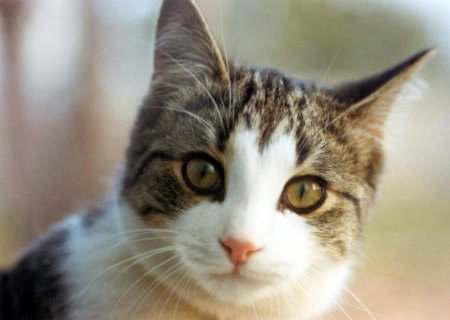
\includegraphics[width=5cm]{cat.jpg}
  \caption{Een kat}
  \label{cat}
\end{figure}

\begin{table}[bp]
  \centering
  \begin{tabular}{l|cr}
    links & gecentreerd & rechts \\ \hline
    links & gecentreerd & rechts \\
  \end{tabular}
  \caption{Een voorbeeldtabel}
  \label{example}
\end{table}
\end{minted}
We gebruiken \emph{modifiers} om de tabellen en figuren op de door ons gewenste plaats te zetten (i.e., een combinatie van \verb|htbp!|).


\section{Wiskunde}
Je moet in \emph{math mode} terechtkomen, waarin \TeX\ totaal anders werkt. Twee opties: via~\mint{tex}|$a^2+b^2=c^2$| of bepaalde omgevingen. Gebruik altijd \mint{tex}|\usepackage{amsmath}|, dan kan je de goede omgevingen gebruiken. We gebruiken \verb|equation| om formules die \'e\'en regel groot zijn te typen, \verb|align| als we een berekening over meerdere regels willen uittypen en op een bepaald symbool willen aligneren en \verb|gather| om meerdere vergelijkingen bij elkaar te zetten.
\begin{minted}[frame=lines]{tex}
\begin{equation}
  \label{pythagoras}
  a^2+b^2=c^2
\end{equation}

\begin{align}
  (x+y)^3 &= (x+y)(x^2+2xy+y^2) \\
  &= (x^3+3x^2y+3xy^2+y^3
\end{align}

\begin{equation*}
  a^2+b^2=c^2
\end{equation*}
\end{minted}
Er is ook telkens een \emph{starred variant}, die niet genummerd wordt. Wil je alignen, maar toch slechts \'e\'en nummer? Gebruik \emph{aligned}
\begin{minted}[frame=lines]{tex}
\begin{equation}
  \begin{aligned}
    (x+y)^3 &= (x+y)(x^2+2xy+y^2) \\
    &= (x^3+3x^2y+3xy^2+y^3
  \end{aligned}
\end{equation}
\end{minted}

Sub- en superscript gebeuren via underscores en hoedjes, dus \mint{tex}|a^n| en \mint{tex}|b_k|. Om meerdere karakters te plaatsen: accolades er rond, dus \mint{tex}|a_{i,j}|. Grieke letters zijn gewoon \mint{tex}|\alpha| en \mint{tex}|\zeta|, hoofdletters zijn \mint{tex}|\Delta|. Als de Griekse letter dezelfde is als de Latijnse bestaat er geen macro. Gebruik \fnurl{Detexify}{http://detexify.kirelabs.org} of de \LaTeX\ symbols list om een symbool te vinden, vaak in een bepaalde package zoals \mint{tex}|\usepackage{amssymb}|. Breuken doe je via \mint{tex}|\frac{}{}|, vierkantswortels met \mint{tex}|\sqrt{5}| en \mint{tex}|\sqrt[3]}{5}|. Sommaties, producties, unies via \mint{tex}|\sum \prod \bigcup|. Haakjes kan je met elkaar laten overeenkomen qua grootte via \mint{tex}|\left(\right)|. Om gewone en vierkantje haakjes te typen, gewoon \mint{tex}|()[]|, de andere gaan via \mint{tex}|\{\}\lfloor\rfloor\lceil\rceil\langle\rangle|.

Matrices analoog aan tabellen, zonder kolomspecificatie:
\begin{minted}[frame=lines]{tex}
\begin{pmatrix}
  1 & 0 \\
  0 & 1
\end{pmatrix}
\end{minted}
Er zijn \verb|matrix| (zonder haakjes), \verb|bmatrix| (vierkante haakjes), \verb|vmatrix| (verticale strepen) en andere.

Lettertypes (gebruik \mint{tex}|\usepackage{amsfonts}| waar nodig):
\begin{center}
  \begin{tabular}{ll}
    commando & resultaat \\\midrule
    \mint{tex}|\mathsf{}| & sans-serif, $\textrm{$k$-}\mathsf{Vect}$ \\
    \mint{tex}|\mathcal{}| & calligraphic, $\mathcal{O}$ \\
    \mint{tex}|\mathfrak{}| & Fraktur, $\mathfrak{m}$ \\
    \mint{tex}|\mathbb{}| & blackboard bold, $\mathbb{R}$ \\
  \end{tabular}
\end{center}


\section{Wijze raad}
Leer documentatie lezen!
\end{document}
